\documentclass[12pt,letterpaper]{article}
\usepackage{fullpage}
\usepackage[top=2cm, bottom=4.5cm, left=2.5cm, right=2.5cm]{geometry}
\usepackage{amsmath,amsthm,amsfonts,amssymb,amscd}
\usepackage{lastpage}
\usepackage{enumerate}
\usepackage{fancyhdr}
\usepackage{mathrsfs}
\usepackage{xcolor}
\usepackage{graphicx}
\usepackage{listings}
\usepackage{hyperref}
\usepackage{tikz-qtree}

\hypersetup{%
  colorlinks=true,
  linkcolor=blue,
  linkbordercolor={0 0 1}
}
 
\renewcommand\lstlistingname{Algorithm}
\renewcommand\lstlistlistingname{Algorithms}
\def\lstlistingautorefname{Alg.}

\lstdefinestyle{Python}{
    language        = Python,
    frame           = lines, 
    basicstyle      = \footnotesize,
    keywordstyle    = \color{blue},
    stringstyle     = \color{green},
    commentstyle    = \color{red}\ttfamily
}

\setlength{\parindent}{0.0in}
\setlength{\parskip}{0.05in}
% Edit these as appropriate
\newcommand\course{CSE 3500}
\newcommand\hwnumber{6}                  % <-- homework number
\newcommand\release{}    % <-- release date
\newcommand\due{}        % <-- homework number

\pagestyle{fancyplain}
\headheight 35pt
\lhead{\course}
\chead{\textbf{\Large Homework \hwnumber}}
\rhead{Released on \release \\ Due on \due}
\lfoot{}
\cfoot{}
\rfoot{\small\thepage}
\headsep 1.5em

\begin{document}

\begin{center}
    \LARGE Competitive Analysis, Greedy and Graph Algorithms
\end{center}

\section*{Problem 0: Birthday Party}

\subsection*{Solution}
\textbf{Task 1}: We can bring 20 kiwis and 2 pineapples. This is because to maximize the
amount of joy without exceeding the weight limit, and knowing the amount of joy that Derek
receives from each fruit, we can maximize the amount of joy by bringing the maximum number
of kiwis and the minimum number of pineapples while being equal parts of each fruit. 

\textbf{Task 2}: The competitive ratio of our algorithm is 2. This is because the oracle can
bring the maximum amount of fruit that Derek can receive joy from, while our algorithm would
only bring half of that making a ratio of 2. Derek can have a scenerio where kiwi is his favorite
fruit while pineapple is only 0. The oracle can bring 40 kiwis and 0 pineapples,
while our algorithm can only bring 20 kiwis and 2 pineapples making it 40 to 20 or a ratio of 2.

\textbf{Task 3}: 
We can find the optimal offline strategy by using the following formula:
\begin{lstlisting}
def optimal(P, K):
    if P > 10k:
      number_of_pineapples = 4
      number_of_kiwis = 0
    else:
      number_of_pineapples = 0
      number_of_kiwis = 40
\end{lstlisting}
This is because if the weight of the pineapple is greater than 10 times the weight of the kiwi,
then we can only bring 4 pineapples. Otherwise, we can only bring 40 kiwis. This would be correct if
we were to bring the maximum amount of joy to Derek as the oracle would maximize the amount
of joy that Derek would receive from only kiwis or only pineapples. 

\textbf{Task 4}: We can show that the competitive ratio is at least 2 by using the same
formula as Task 3. We can show that the oracle can bring 40 kiwis and 0 pineapples
or 0 kiwis and 4 pineapples. This would be correct as we would bring the maximum amount of
joy to Derek. From the algorithm of bringing 20 kiwis and 2 pineapples, we can see that the
competitive ratio is 2 as the orcale would bring the maximum amount of joy to Derek while our
algorithm would bring half of that making a ratio of 2.

\textbf{Task 5a}: We can show that the special case of K = 0 and P = 0 yields a joy upper
bounded by 2 by again using the same formula as Task 3 and our algorithm. We can show that
the oracle can still bring either 40 kiwis and 0 pineapples or 0 kiwis and 4 pineapples and our
algorithm would still bring 20 kiwis and 2 pineapples. The ratio would still be 2 as the oracle
would bring the maximum amount of joy to Derek while our algorithm would bring half of that.

\textbf{Task 5b}: We can show that the competitive ratio is at most 2 by using the same
formula as Task 3. We can show that the oracle can bring 40 kiwis and 0 pineapples
or 0 kiwis and 4 pineapples. This would be correct as we would bring the maximum amount of
joy to Derek. From the algorithm of bringing 20 kiwis and 2 pineapples, we can see that the
competitive ratio is 2 as the orcale would bring the maximum amount of joy to Derek while our
algorithm would bring half of that making a ratio of 2.




\section*{Problem 1: Matryoshka dolls}

In this problem, we are given a backpack of capacity $Z$ and a a set of matryoshka dolls.
We are interested in the maximum value of the dolls that we can fit in the backpack without
exceeding the capacity. Each doll has a index $i$, a weight $w_i$, and a value $v_i$. We
can only take one of each doll. To solve this problem, with a greedy algorithm, we will
first order the dolls by their index. From there, we will get the profit per unit weight of
each doll and have them be in the same order as the index. We will then choose the doll
with the highest profit per unit weight. When we choose it, we will subtract its weight from
the capacity of the backpack. We will continue to choose the doll with the highest profit
per unit weight until we reach the capacity of the backpack, each time we choose we would
mark down with a 1, if it was not chosen we would mark it with a 0. If there is space left in the
backpack, but the doll has a weight that is greater than the capacity of the backpack,
we would still choose that doll, but we would only take a fraction of it and mark it with that fraction. 
This is because we want to maximize the value of the dolls that we take. In the end, we will have a set of
dolls with a 1 or a fraction that we will take. We can now calculate the value of the dolls
that we will take by multiplying the value of the doll by the fraction that we will take. We
will then add all of the values together to get the total value of the dolls that we will take
which is the maximum value of the dolls that we can fit in the backpack without exceeding
the capacity.
\begin{enumerate}
  \item We first order the dolls by their index. We then get the profit per unit weight of
each doll and have them be in the same order as the index. 
  \item We then choose the doll with the highest profit per unit weight. When we choose it, we
subtract its weight from the capacity of the backpack. 
  \item We repeat step 2 until we reach the capacity of the backpack, each time we choose we
would mark down with a 1, if it was not chosen we would mark it with a 0. If there is space
left in the backpack, but the doll has a weight that is greater than the capacity of the
backpack, we would still choose that doll, but we would only take a fraction of it and mark
it with that fraction. 
  \item We then calculate the value of the dolls that we will take by multiplying the value of
the doll by the fraction that we will take. We will then add all of the values together to
get the total value of the dolls.
\end{enumerate}

We can assume that this is the most optimal solution because we are choosing the doll with
the highest profit per unit weight. If we were to choose a doll with a lower profit per unit
weight, we would be losing out on profit. If we were to choose a doll with only by
profit, we would not be maximizing the value of the dolls that we take. 
For example, if we had 7 dolls with the following values:
\begin{itemize}
  \item Doll 1: value = 10, weight = 2
  \item Doll 2: value = 5, weight = 3
  \item Doll 3: value = 15, weight = 5
  \item Doll 4: value = 7, weight = 7
  \item Doll 5: value = 6, weight = 1
  \item Doll 6: value = 18, weight = 4
  \item Doll 7: value = 3, weight = 1
\end{itemize}
If we were to choose the doll with the highest profit per unit weight, we would choose 
dolls [1, 2/3 of 2, 3, 5, 6, 7]. This would give us a total value of 
54.6. If we only chose dolls by value, we would choose dolls [1, 3, 4/7 of 4, 6] which would
give us 22 value. This is not the optimal solution because we are losing out on profit. Therefore,
we can assume that this is the most optimal solution.

\section*{Problem 2: Min-cuts}

\subsection*{1.}
We can observe that:
\begin{enumerate}
  \item S has a outflow of 1 into a, b, and c making the total outflow of S 3.
  \item a has a inflow of 1 from S and an outflow of 1 into b and t
  \item b has a inflow of 1 from a and S and an outflow of 1 into c and t
  \item c has a inflow of 1 from b and S and an outflow of 1 into t
  \item t has a inflow of 1 from a, b, and c making the total inflow of t 3.
\end{enumerate}
We can see that a has more outflow than inflow but can only outflow 1, b has the same amount of outflow and inflow, and
c has more inflow than outflow. Since all the edges have a capacity of 1 and are all equal, we can assume that the
min-cut is 3. 

\subsection*{2.}
We can observe that:
\begin{enumerate}
  \item S has a outflow of 2, 3, and 4 into a, b, and c making the total outflow of S 9.
  \item a has a inflow of 2 from S and an outflow of 5 and 4 into b and t
  \item b has a inflow of 3 and 5 from S and a 5 and 3 into c and t
  \item c has a inflow of 4 and 5 from S and b and an outflow of 2 into t
  \item t has a inflow of 4, 3, and 2 from a, b, and c making the total inflow of t 9.
\end{enumerate}
From this we would make cuts at 2, 3, and 2. This would give us a min-cut of 7.

\subsection*{1.}
\begin{center}
  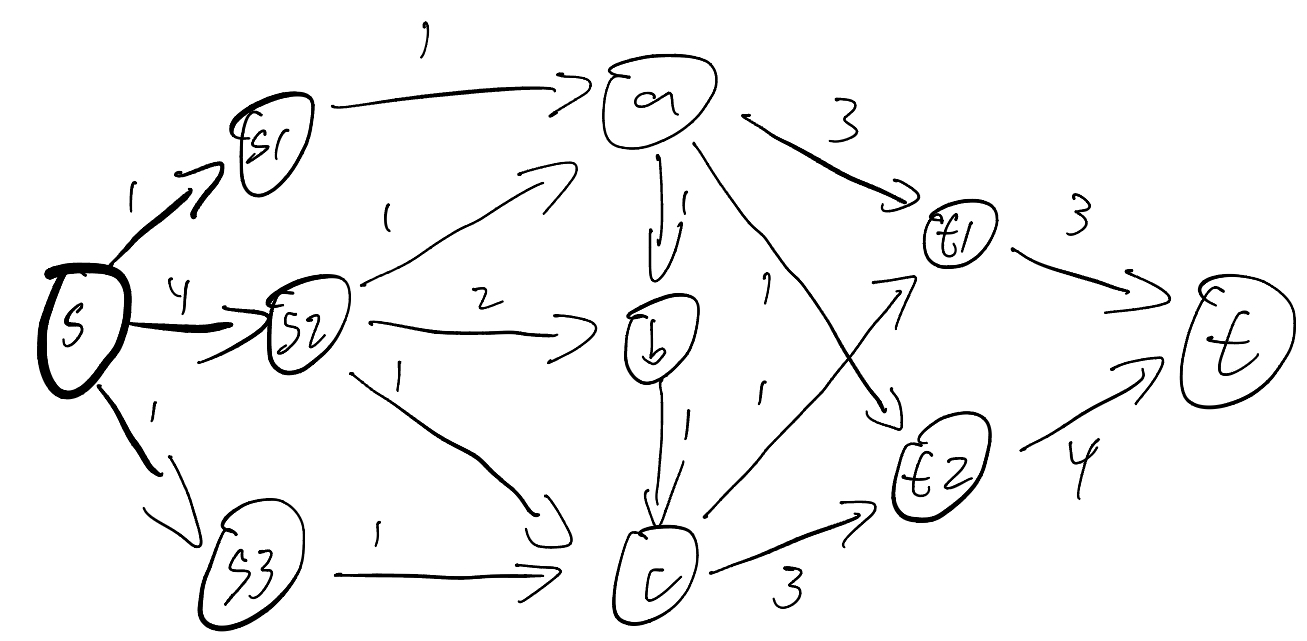
\includegraphics[scale = .35]{./images/3.1.jpeg}
\end{center}
I would add a source node that flows into s1, s2, and s3. I would then add
a sink node inflows t1 and t2.

\subsection*{2.}
I would add a source node that flows into each resident. I would then add a sink node
that flows from each hospital. I would then add edges from each resident to each hospital
with a capacity of 1. I would then add edges from each hospital to the sink node with a
capacity of 3. The maximum cardinality matching would be the minimum cut of the graph.
This would also be the maximum flow of the graph. 
I would then use the Ford-Fulkerson algorithm to find the maximum flow of the graph. 
The Ford-Fulkerson algorithm runs in $O(VE^2)$ time, where $V$ is the number of vertices
and $E$ is the number of edges. Therefore, the algorithm would run in polynomial time.

\end{document}
